Analizziamo ora le caratteristiche dello strumento che ci permette di misurare i fotoni (e, quindi, la luce) emessi da una stella che desideriamo studiare: il telescopio.

Il compito dei telescopi è quello di raccogliere la radiazione che arriva dallo spazio e riunirla in un unico punto. La storia ci dice che Galileo non inventò il telescopio, ma che comunque fu il primo ad utilizzarlo per condurre misure astronomiche.

Se decidessimo di graficare un istogramma del numero di fotoni che arrivano su un determinato telescopio in ogni intervallo di tempo, ci accorgeremmo subito che la statistica che domina questo fenomeno è la \textit{statistica di Poisson}. Questa afferma che per $N$ eventi indipendenti (in questo caso, l'arrivo di un fotone) in un dato intervallo di tempo, la probabilità di osservarne $n$ è di

\begin{equation*}
    P_N(n) = \frac{N^n}{n!}e^{-N}
\end{equation*}

Allora, se $N$ è il valore medio del numero di fotoni che sono arrivati sul nostro telescopio, l'errore su questo conteggio secondo Poisson è dato dalla radice quadrata della media: $\sqrt{N}$. L'errore relativo sarà, quindi,

$$\frac{\sqrt{N}}{N} = \frac{1}{\sqrt{N}}$$

Gli astrofisici preferiscono comunque calcolare la qualità della misura come l'inverso dell'errore relativo, frazione che corrisponde al cosiddetto \textbf{rapporto segnale su rumore}:

\begin{equation}
    \frac{\text{Signal}}{\text{Noise}} = \sqrt{N}
\end{equation}

Il telescopio costruito da Galileo, detto \textbf{rifrattore}, si basava sull'utilizzo di due lenti di vetro: la \textit{lente primaria}, convergente, aveva il compito di raccogliere i raggi del fronte d'onda piano incidente e convogliarli verso il fuoco, formando un'immagine puntiforme; la seconda lente, detta \textit{oculare} e divergente, ritrasformava l'immagine puntiforme in un fronte d'onda piano che poteva essere visto dall'occhio. L'utilità della prima lente stava nel raccogliere molti più fotoni rispetto alla quantità di cui sarebbe stato capace l'occhio umano da solo. Veniva così amplificato il segnale di una stella.

\begin{figure}[H]
    \centering
    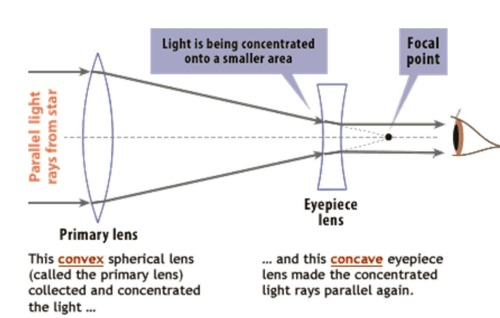
\includegraphics[width=8cm]{WhatsApp Image 2023-01-09 at 02.42.01.jpeg}
    \label{fig:my_label4}
\end{figure}

Il telescopio proposto da Newton, detto \textbf{riflettore}, invece usava uno specchio ricurvo per convogliare i raggi di luce verso un secondo specchio, inclinato di 45 gradi rispetto alla focale, che li rifletteva tutti in un punto ben preciso.

\begin{figure}[H]
    \centering
    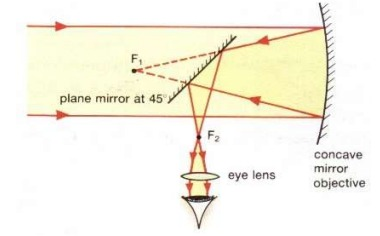
\includegraphics[width=8cm]{WhatsApp Image 2023-01-09 at 02.44.03.jpeg}
    \label{fig:my_label5}
\end{figure}

In ogni caso, ciò che caratterizza un telescopio è il diametro $D$ del suo specchio primario (o della sua lente primaria); infatti, il numero di fotoni $N$ raccolti da un telescopio è proporzionale all'area di tale specchio e, quindi, a $D^2$.

Allora, se il rapporto segnale/rumore è

$$\frac{Signal}{Noise}=\sqrt{N}
\quad\text{e}\quad
N \propto D^2$$

il rapporto segnale rumore risulterà proporzionale al diametro $\frac{signal}{noise} \propto D$. Per cui, raddoppiare il diametro significa ricevere il quadruplo dei fotoni e dunque raddoppiare la qualità della misura.

Alternativamente, se si vuole migliorare la qualità della misura avendo un diametro fisso, essendo il numero di fotoni $N$ lineare nel tempo $T_{exp}$, si può pensare di esporre il telescopio più a lungo alla sorgente luminosa, aumentando il numero di fotoni cosi rivelati. Ovviamente, più è grande il diametro, meno tempo si impiegherà a raccogliere il numero $N$ di fotoni desiderato.

Facciamo un esempio numerico: il telescopio di Serra la Nave ha un diametro di 1 m, mentre i telescopi costruiti oggigiorno hanno diametro di 8 m. Per rivelare lo stesso numero di fotoni che un telescopio di quest'ultimo tipo rivela in un minuto, quello di Serra la Nave dovrà essere esposto per 64 minuti, cioè circa un'ora.

\subsubsection{Proprietà di un telescopio}

Le caratteristiche di un sistema ottico utili per descrivere un telescopio sono:

\begin{itemize}
    \item $D=2R$ apertura;
    \item $V$ vertice identificato dall'asse di simmetria, rispetto al quale si misurano anche angoli;
    \item $f$ distanza focale, dove la radiazione viene raccolta;
    \item $F$ fuoco;
    \item $Q$ fuoco per $\alpha$ (vedi sotto);
    \item $FQ$ piano focale;
    \item $\alpha f$ distanza dell'immagine.
\end{itemize}

\begin{figure}[H]
    \centering
    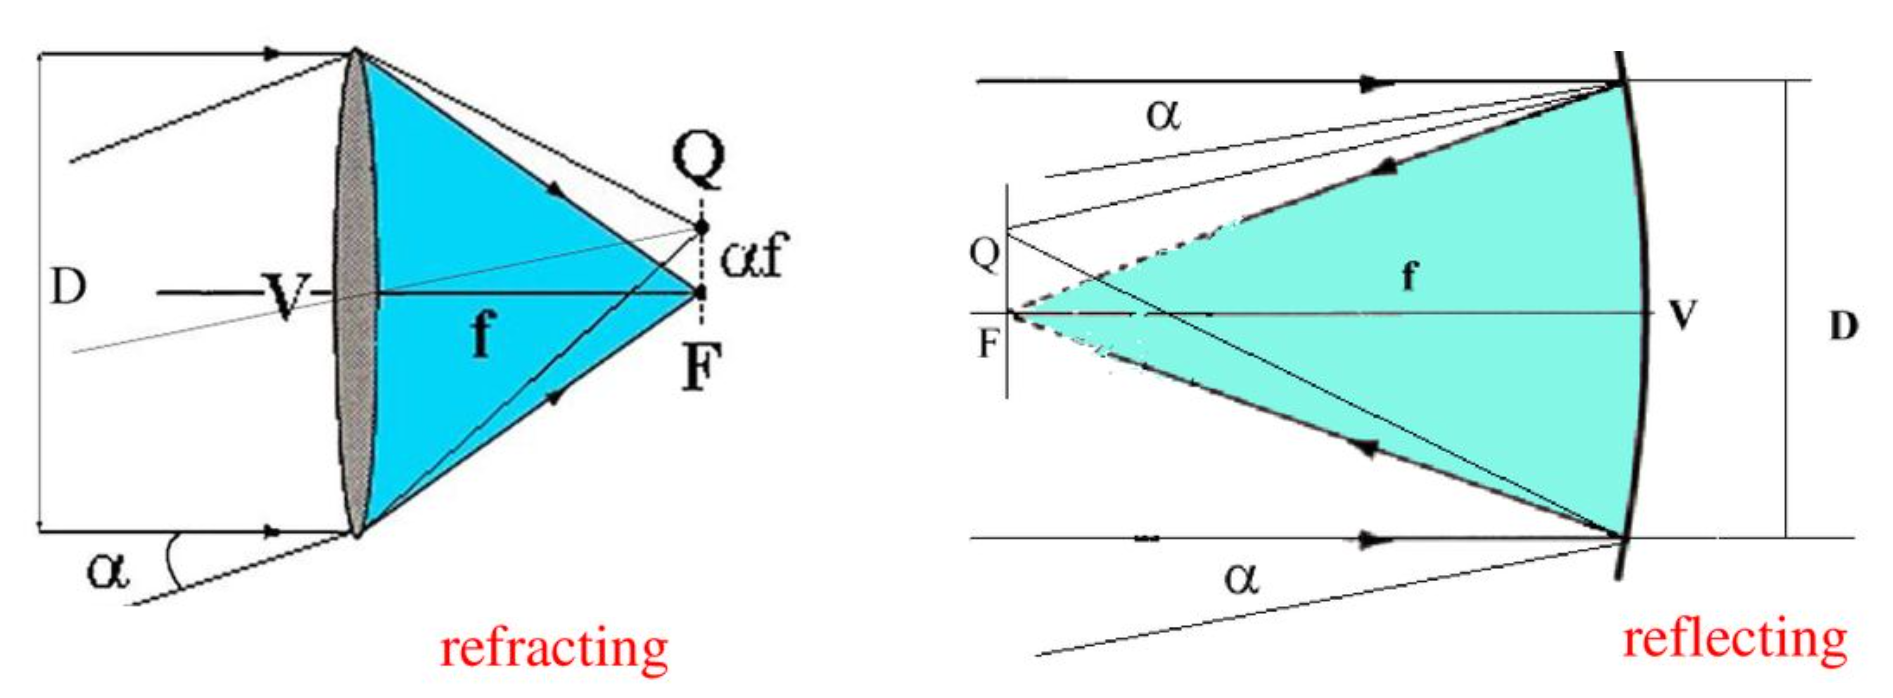
\includegraphics[width=12cm]{immagini/proprieta_telescopi_1.png}
\end{figure}


%\begin{figure}[H]
%    \centering
%    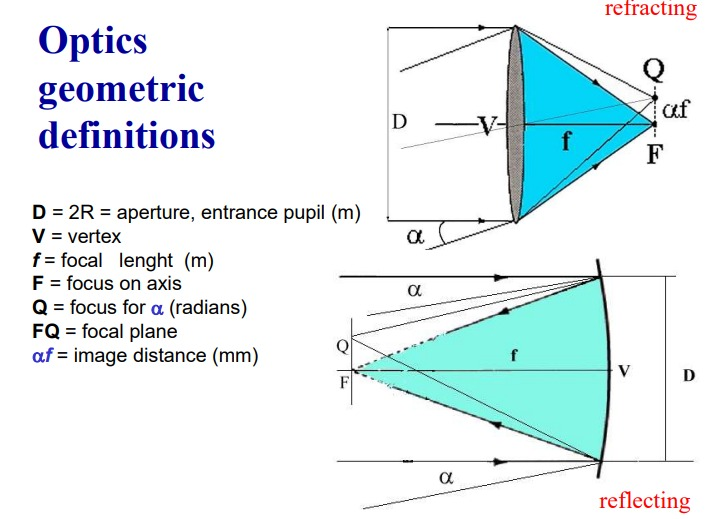
\includegraphics[width=8cm]{WhatsApp Image 2023-01-09 at 02.46.32.jpeg}
%    \label{fig:my_label6}
%\end{figure}

Il fuoco, in particolare, rappresenta il punto sull'asse ottico in cui tutti i raggi incidenti paralleli all'asse ottico vengono convogliati dalla lente o dallo specchio del telescopio. Nel caso in cui i raggi incidenti dell'oggetto osservato siano inclinati di un certo angolo $\alpha$ rispetto alla direzione dell'asse ottico, l'immagine si formerà in un punto $Q$ (diverso dal fuoco) giacente sul cosiddetto \textbf{piano focale} e distante dal fuoco $f \sin{\alpha} \simeq f\alpha$.

Quanto sarà grande il piano focale? Il fattore di scala di questo piano sarà dato da un radiante espresso in arcosecondi diviso la focale espressa in millimetri, cioè

\begin{equation*}
    \frac{206264.8062''}{f}
\end{equation*}

Quindi, ad esempio, se il telescopio ha una focale di 16 metri, una stella di ampiezza 1 arcosecondo sarà grande su questo telescopio $0.388$ mm. \textbf{SI MA STA COSA NON HO IDEA DI COME ESCA}

Allora, se per il diametro del telescopio è facile affermare in generale che più grande è e meglio è, per la focale la grandezza va decisa in base alle misure che lo sperimentatore vuole condurre (di una singola stella come della luna), poiché cambierà il modo in cui gli oggetti verranno visualizzati.

Definiamo poi \textbf{campo di vista} la quantità di cielo che un telescopio può osservare contemporaneamente. Quantitativamente, è l'angolo $\varphi$ che il "raggio principale" (cioè quel raggio che si propaga attraverso la lente senza essere rifratto) può sottendere data l'apertura dell'oculare da cui l'occhio osserva l'immagine. I telescopi moderni hanno un campo di vista nell'ordine degli arcominuti.

\begin{figure}[H]
    \centering
    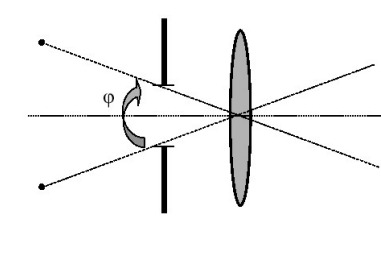
\includegraphics[width=5cm]{WhatsApp Image 2023-01-09 at 02.51.58.jpeg}
    \label{fig:my_label7}
\end{figure}

Vi è poi Il \textbf{potere risolutivo}, che è l'abilità di un telescopio di separare due oggetti, ad esempio due stelle in cielo che distano l'una dall'altra di un certo angolo. L'angolo di distanza più piccolo a cui il telescopio riesce a distinguere due oggetti è detto \textbf{risoluzione angolare}.

Per capire cosa sia davvero il potere risolutivo analizziamo l'esperimento della doppia fenditura.

\begin{minipage}{0.68\textwidth}
    Quando una radiazione elettromagnetica incide sulla piccola fenditura che è l'apertura del telescopio, secondo il principio di Huygens, ogni punto della fenditura stessa diventa una nuova sorgente di fronte d'onda circolare. Questi fronti si sovrappongono, formando una nuova onda risultante che può essere descritta come la trasformata di Fourier del prodotto delle funzioni $E(x,t) = E_0e^{i(kx-\omega t)}$, espressione dell'onda piana incidente, e la funzione di trasmissione del telescopio definita a tratti come $G(x) = 1$ se $x$ individua un punto dentro l'apertura e $G(x)=0$ altrimenti.

    La quantità di luce in una direzione $\beta$ è data dall'integrale
    $$g(\beta)=\int_{-\infty}^{+\infty} E(x) G(x) e^{2 \pi i (x/\lambda) \sin \beta} \; dx$$
\end{minipage}
\begin{minipage}{0.315\textwidth}
    \begin{figure}[H]
        \centering
        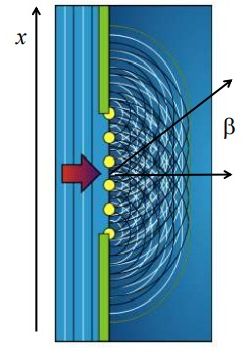
\includegraphics[width=5cm]{immagini/diffrazione.png}
        \label{fig:my_label8}
    \end{figure}
\end{minipage}

Sostituendo la media temporale dell'onda incidente che è $E(x)=E_0 e^{2 \pi i (x/\lambda)}$ otteniamo

$$g(\beta)=E_0 \int_{-\infty}^{+\infty} G(x) e^{2 \pi i (x/\lambda) \sin \beta} \; dx$$

Questa nuova funzione ci darà il valore dell'onda in una qualunque direzione descritta dalla coordinata spaziale $\beta$ o dalla coordinata angolare $\theta$. Se scriviamo $x$ in unità di lunghezza d'onda $\lambda$, e poniamo $\theta=\sin{\beta}$ otteniamo

\begin{equation*}
    g(\theta) = E_0 \int_{-\infty}^{+\infty} G(x)e^{2ix\pi\theta} \; dx
\end{equation*}

che è la trasformata di Fourier della trasmittanza $G(x)$. Svolgendo tale integrale si ottiene la funzione seno circolare

$$g(\theta)=E_0 \frac{sin(\pi t)}{\pi t}$$

\rule[7pt]{\linewidth}{0.4pt}

Mostriamo esplicitamente come si giunge a tale risultato.

Ricordiamo la funzione boxcar

\begin{minipage}{0.5\textwidth}
    $$h(x)=
    \begin{cases}
        1 & \text{per } -1<x<1\\
        0 & \text{per } x \leq -1 \vee x \geq 1
    \end{cases}$$
\end{minipage}
\begin{minipage}{0.5\textwidth}
    \begin{figure}[H]
        \centering
        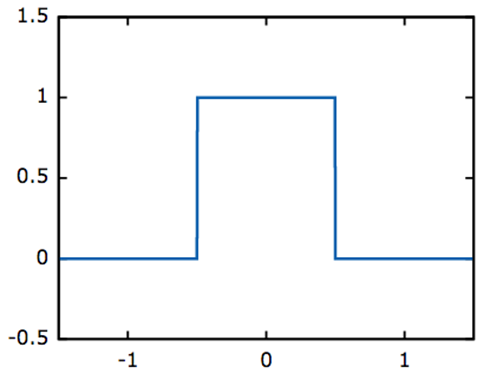
\includegraphics[width=4cm]{immagini/funzione_boxcar.png}
    \end{figure}
\end{minipage}

La trasformata di Fourier di tale funzione sarà

$$H(t)=\int_{-\infty}^{+\infty} h(x) e^{2 \pi i tx} \; dx
=\int_{-1}^{1} e^{2 \pi i tx} \; dx
=\left[ \frac{e^{2 \pi i tx}}{2 \pi i t} \right]_{-1}^{1}=$$
$$=\frac{1}{2\pi i t} \left[ e^{2 \pi i t} - e^{-2 \pi i t} \right]
=\frac{\sin{(\pi t)}}{\pi t}$$

\rule[7pt]{\linewidth}{0.4pt}

Se un'onda piana investe un telescopio, sul piano focale si osserverà tale figura:

\begin{figure}[H]
    \centering
    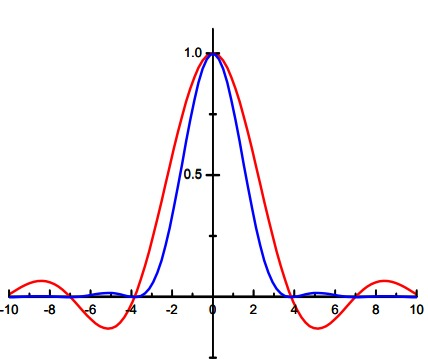
\includegraphics[width=5cm]{WhatsApp Image 2023-01-09 at 02.57.58.jpeg}
    \label{fig:my_label9}
\end{figure}

Dove sulle ordinate abbiamo la luminosità e sulle ascisse la distanza \textbf{espressa in angoli??}.

Dal grafico deduciamo che al centro della fenditura ci sarà molta luce; allontanandoci da essa, la luce sarà meno intensa fino a che spunteranno altri picchi luminosi (anche questi meno intensi del picco principale) in corrispondenza di precisi punti.

Considerando che l'apertura del telescopio non è una semplice striscia, ma presenta una forma circolare, l'immagine che si otterrà, detta \textbf{disco di Airy} e descritta dalla funzione di Bessell, è la seguente:

\begin{figure}[H]
    \centering
    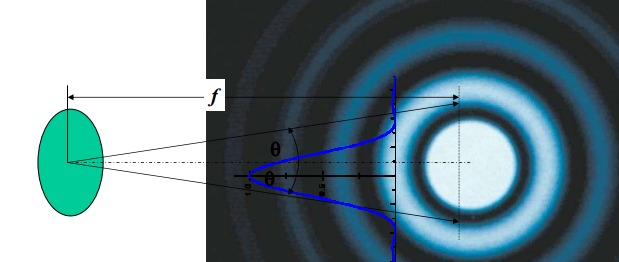
\includegraphics[width=10cm]{WhatsApp Image 2023-01-09 at 02.59.37.jpeg}
    \label{fig:my_label10}
\end{figure}

Si dimostra che il picco dello spettro (il centro, corrispondente alla parte più luminosa) viene collimato nel centro dell'apertura circolare del telescopio quanto più è grande il diametro $D$ del telescopio stesso. Infatti, chiamando $\theta$ l'angolo di distanza tra i due centri (vedi figura sopra) si ha $\sin{\theta}=\frac{1.22\lambda}{D}$ per il primo picco. Più cresce $D$, più il seno tenderà a zero e, quindi, più $\vartheta$ sarà approssimabile a zero (sovrapposizione). Per cui, più un telescopio è grande, più ci aspettiamo che la larghezza dello spettro prodotto da una stella sia piccola.

Quindi il vantaggio di avere un telescopio di diametro ampio non è solo quello di ricevere più fotoni, ma soprattutto quello di produrre immagini più nitide.

Che intendiamo per nitide? Immaginiamo di osservare due stelle molto vicine:

\begin{figure}[H]
    \centering
    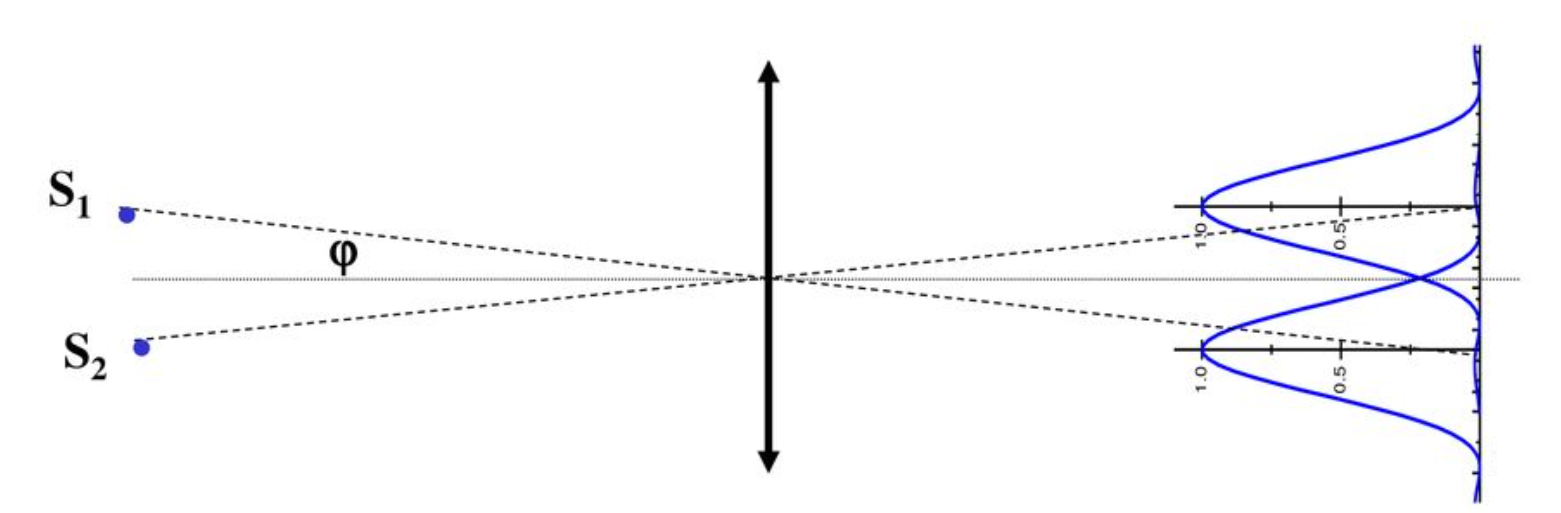
\includegraphics[width=12cm]{immagini/spettri_due_stelle.png}
\end{figure}

I due spettri prodotti da esse (considerando che presentano una certa larghezza dipendente dal diametro del telescopio) potrebbero sovrapporsi, per cui è lecito chiedersi in che condizioni il telescopio riuscirà a distinguere le due stelle. Se la separazione dei picchi dipende dalla risoluzione angolare $\phi$ del telescopio, il diametro del telescopio determinerà invece quanto le larghezze dei due spettri saranno grandi e, quindi, quanto essi si sovrapporranno o meno. Il \textbf{criterio di Rayleigh} stabilisce una condizione oggettiva: due sorgenti si potranno ritenere distinte se lo zero della prima sorgente cade sul massimo della seconda sorgente. L'argomento in dettaglio si trova nelle slide di Costa del terzo ciclo.